% asset_id: OffSpecNumericalMethodsTikZ-003
% source: AI-proposed Simpson's rule labelling diagram based on supplied evidence
% status: Off-spec enrichment, not CCEA Further Mathematics core
\documentclass[tikz,border=8pt]{standalone}
\usepackage{amsmath}\usetikzlibrary{arrows.meta}
\definecolor{Canvas}{HTML}{FAF9F6}\definecolor{Ivory}{HTML}{FFFFF0}\definecolor{LineGrey}{HTML}{E5E5EA}\definecolor{AccentGold}{HTML}{C5A059}\definecolor{SoftPink}{HTML}{FBEFEF}\definecolor{TextMath}{HTML}{2C2C2E}
\begin{document}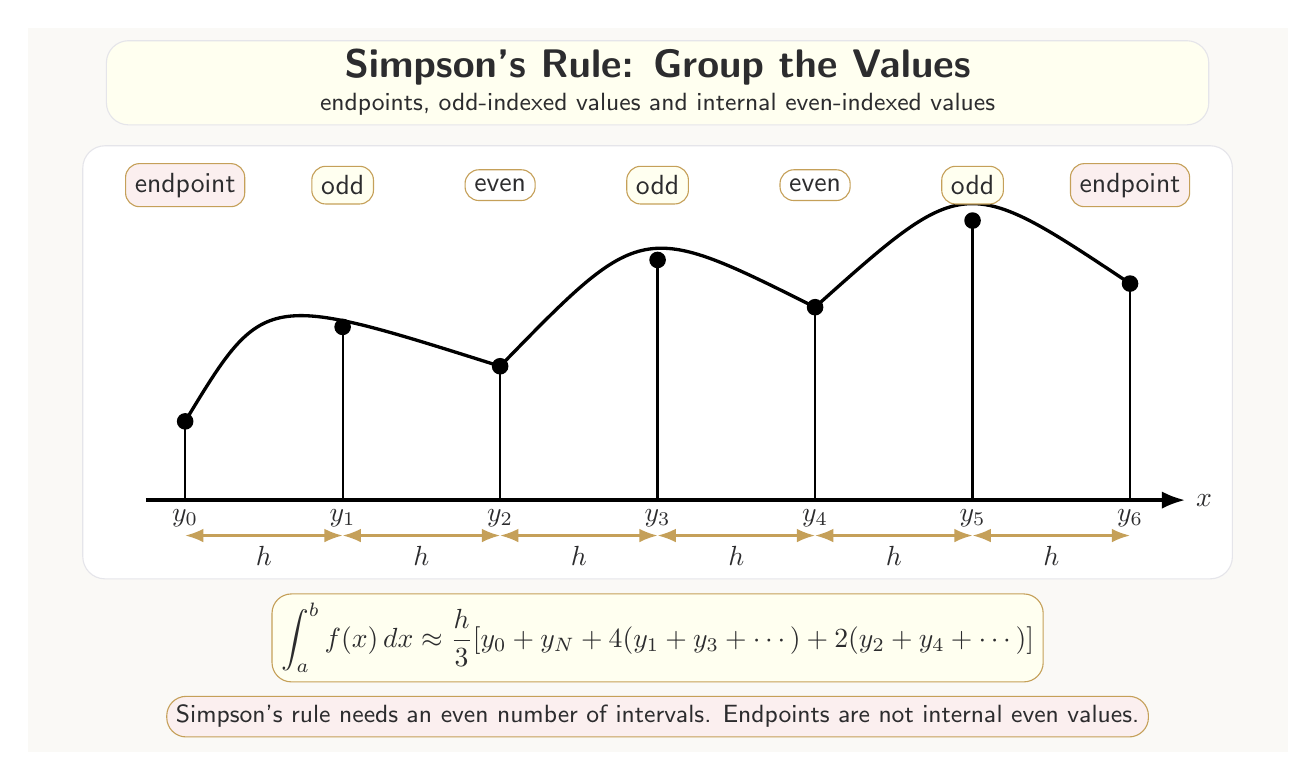
\begin{tikzpicture}[>=Latex,every node/.style={font=\sffamily,text=TextMath}]
\fill[Canvas](-1,-1.2)rectangle(15,8);\node[draw=LineGrey,fill=Ivory,rounded corners=8pt,minimum width=14cm,minimum height=1cm,align=center]at(7,7.3){\Large\textbf{Simpson's Rule: Group the Values}\\\small endpoints, odd-indexed values and internal even-indexed values};
\draw[draw=LineGrey,fill=white,rounded corners=8pt](-.3,1)rectangle(14.3,6.5);\draw[->,very thick](.5,2)--(13.7,2)node[right]{$x$};
\foreach \x/\y/\lab in {1/3/y_0,3/4.2/y_1,5/3.7/y_2,7/5.05/y_3,9/4.45/y_4,11/5.55/y_5,13/4.75/y_6}{\draw[thick](\x,2)--(\x,\y);\fill(\x,\y)circle(3pt);\node[below]at(\x,2){$\lab$};}
\draw[very thick](1,3)..controls(2,4.65)..(5,3.7)..controls(6.8,5.55)..(9,4.45)..controls(10.9,6.15)..(13,4.75);
\foreach \a/\b in {1/3,3/5,5/7,7/9,9/11,11/13}{\draw[<->,AccentGold,thick](\a,1.55)--(\b,1.55)node[midway,below]{$h$};}
\node[draw=AccentGold,fill=SoftPink,rounded corners=5pt]at(1,6){endpoint};\node[draw=AccentGold,fill=SoftPink,rounded corners=5pt]at(13,6){endpoint};\node[draw=AccentGold,fill=Ivory,rounded corners=5pt]at(3,6){odd};\node[draw=AccentGold,fill=Ivory,rounded corners=5pt]at(7,6){odd};\node[draw=AccentGold,fill=Ivory,rounded corners=5pt]at(11,6){odd};\node[draw=AccentGold,fill=white,rounded corners=5pt]at(5,6){even};\node[draw=AccentGold,fill=white,rounded corners=5pt]at(9,6){even};
\node[draw=AccentGold,fill=Ivory,rounded corners=7pt,align=center]at(7,.25){$\displaystyle \int_a^b f(x)\,dx\approx\frac{h}{3}[y_0+y_N+4(y_1+y_3+\cdots)+2(y_2+y_4+\cdots)]$};
\node[draw=AccentGold,fill=SoftPink,rounded corners=7pt,align=center]at(7,-.75){\small Simpson's rule needs an even number of intervals. Endpoints are not internal even values.};
\end{tikzpicture}\end{document}
